\documentclass[11pt,twocolumn]{article}

% --- Packages ---
\usepackage[utf8]{inputenc}
\usepackage[T1]{fontenc}
\usepackage{amsmath,amssymb}
\usepackage{graphicx}
\usepackage{booktabs}
\usepackage{multirow}
\usepackage{hyperref}
\usepackage[margin=1in]{geometry}
\usepackage{caption}
\usepackage{subcaption}
\usepackage{xcolor}
\usepackage{algorithm}
\usepackage{algorithmic}
\usepackage{cite}
\usepackage{url}
\usepackage{tabularx}

\graphicspath{{figures/}}

% --- Title ---
\title{LLM-Guided Bayesian Optimization for Nuclear Reactor Control Rod Positioning: A Benchmark Against Classical Controllers}

\author{
  % Authors omitted for review
}

\date{}

\begin{document}

\maketitle

% ============================================================
% ABSTRACT
% ============================================================
\begin{abstract}
We present a novel agentic control framework that couples a large language model (LLM) with Gaussian process Bayesian optimization (BO) for nuclear reactor control rod positioning.
The LLM proposes candidate rod positions informed by reactor state history, while the BO module scores each candidate via a safety-aware acquisition function with asymmetric penalties for supercritical deviations.
We benchmark this LLM+BO controller against enhanced PID and proportional-only baselines across ten PWR pin-cell configurations simulated with OpenMC Monte Carlo transport.
The classical baselines incorporate gain scheduling based on online rod worth estimation, dead-band suppression for limit cycle prevention, and continuous (float) rod positioning---representing a state-of-the-art classical control implementation.
Despite these enhancements, the LLM+BO controller achieves superior convergence rates and tighter $k_\text{eff}$ regulation, demonstrating that LLM-guided search constrained by a physics-informed surrogate can outperform well-tuned classical feedback controllers in the inherently nonlinear control rod worth landscape.
\end{abstract}

% ============================================================
% 1. INTRODUCTION
% ============================================================
\section{Introduction}
\label{sec:introduction}

Maintaining reactor criticality ($k_\text{eff} = 1.0$) through control rod manipulation is a fundamental task in nuclear reactor operation.
The relationship between control rod insertion depth and reactivity is governed by the differential rod worth curve, which exhibits a characteristic S-shape: rod worth is low near fully inserted and fully withdrawn positions and peaks near the core midplane~\cite{duderstadt1976nuclear,glasstone2012nuclear}.
This nonlinearity poses a significant challenge for classical linear feedback controllers, as the same control signal produces vastly different reactivity effects depending on the operating point.

Proportional-Integral-Derivative (PID) controllers have long served as the standard approach for reactor power regulation~\cite{cho2012nuclear}.
However, PID tuning assumes locally linear plant dynamics, and the fixed-gain structure struggles with the S-curve nonlinearity of control rod worth.
In practice, gain scheduling or adaptive schemes are employed, but these add complexity and require explicit plant models.

Recent advances in large language models (LLMs) have demonstrated their capacity for reasoning over sequential decision-making tasks~\cite{brown2020language,touvron2023llama}.
Concurrently, Bayesian optimization (BO) with Gaussian process (GP) surrogates has proven effective for sample-efficient optimization of expensive black-box functions~\cite{shahriari2016taking,snoek2012practical}.
We hypothesize that an LLM can serve as an informed proposal generator---leveraging its capacity to reason about reactor physics from contextual state descriptions---while a GP surrogate provides a principled safety scoring mechanism grounded in observed simulation data.

In this work, we introduce an \emph{agentic} control framework where:
\begin{enumerate}
    \item A locally deployed LLM (Qwen3.5-9B) generates candidate control rod target positions based on the current reactor state and operational history.
    \item A GP-based Bayesian optimizer scores each candidate using an asymmetric safety penalty that is stricter for supercritical deviations.
    \item The highest-scoring candidate is executed in an OpenMC Monte Carlo simulation, and the result is used to refit the GP surrogate.
\end{enumerate}

We benchmark this LLM+BO controller against enhanced PID ($K_p\!=\!40$, $K_i\!=\!8$, $K_d\!=\!3$, gain scheduling, dead-band) and proportional-only ($K_p\!=\!40$, gain scheduling) controllers across all ten PWR pin-cell blueprints.
Both classical and LLM+BO controllers use continuous (float) rod positions, ensuring a fair comparison.
Our results show that the LLM+BO approach achieves higher convergence rates and lower $k_\text{eff}$ deviations, with best-case performance reaching $|\Delta k_\text{eff}| < 0.001$.

% ============================================================
% 2. RELATED WORK
% ============================================================
\section{Related Work}
\label{sec:related}

\subsection{Classical Reactor Control}

Reactor power control has traditionally relied on PID-based feedback systems operating on neutron flux or power error signals~\cite{duderstadt1976nuclear}.
The nonlinear relationship between rod position and reactivity has motivated gain-scheduling approaches, where PID gains are adjusted as a function of rod position or power level~\cite{cho2012nuclear}.
Mousakazemi~\cite{mousakazemi2019scheduled} demonstrated a scheduled PID controller for PWR core power using gains optimized by genetic algorithms, while Eliasi~\cite{eliasi2019antiwindup} addressed control rod speed saturation with dynamic anti-windup compensation.
Model predictive control (MPC) has also been explored for reactor load-following, offering constraint handling at the cost of requiring an accurate plant model~\cite{eliasi2011robust}.

\subsection{Machine Learning in Nuclear Engineering}

Machine learning applications in nuclear engineering have expanded rapidly.
Neural networks have been applied to reactor diagnostics~\cite{uhrig1999nuclear}, fuel performance prediction, and neutronics surrogate modeling.
Deep reinforcement learning has been explored for reactor control, where agents learn control policies through interaction with simulation environments~\cite{radaideh2021physics}.
GP surrogates have been used for uncertainty quantification in nuclear simulations, leveraging their natural uncertainty estimates~\cite{wu2018kriging}.

\subsection{LLM Applications in Engineering}

Large language models have recently been applied to scientific reasoning and engineering optimization.
LLMs have demonstrated the ability to propose experimental designs~\cite{boiko2023autonomous}, generate optimization candidates~\cite{yang2024large}, and serve as components in agentic systems that interact with external tools~\cite{schick2023toolformer}.
However, to our knowledge, no prior work has applied LLMs to nuclear reactor control rod optimization.

\subsection{Bayesian Optimization}

Bayesian optimization with GP surrogates is a well-established framework for sample-efficient optimization of expensive black-box functions~\cite{shahriari2016taking,snoek2012practical}.
The GP provides both a mean prediction and uncertainty estimate, enabling principled exploration--exploitation trade-offs through acquisition functions such as Expected Improvement (EI) or Upper Confidence Bound (UCB).
In our work, we use a custom safety-aware acquisition function rather than standard EI, as the objective is to reach a target $k_\text{eff}$ rather than to minimize or maximize an unbounded function.

% ============================================================
% 3. METHODOLOGY
% ============================================================
\section{Methodology}
\label{sec:methodology}

\subsection{System Architecture}

Our system follows a modular, loosely coupled architecture orchestrated through a simulation pipeline (Figure~\ref{fig:architecture}).
The pipeline consists of four layers:

\begin{itemize}
    \item \textbf{ARMI Layer}: Manages case configurations, folder structures, parameter sweeps, and result collection using Pydantic data models for type-safe data exchange.
    \item \textbf{OpenMC Layer}: Generates XML input files from case configurations, executes Monte Carlo transport simulations, and parses statepoint results.
    \item \textbf{Run Manager}: Handles OpenMC process execution with environment variable configuration (OMP\_NUM\_THREADS), timeout management, and retry logic.
    \item \textbf{Controller Layer}: Implements the control logic. The \texttt{BaseController} abstract class defines the interface: \texttt{propose\_actions()}, \texttt{apply\_actions\_to\_case()}, \texttt{evaluate\_results()}, and \texttt{update\_state()}.
\end{itemize}

The control loop proceeds as:
\begin{equation}
    \text{State} \xrightarrow{\text{propose}} \text{Actions} \xrightarrow{\text{apply}} \text{CaseConfig} \xrightarrow{\text{simulate}} \text{Result} \xrightarrow{\text{evaluate}} \text{State}'
\end{equation}

\begin{figure*}[t]
    \centering
    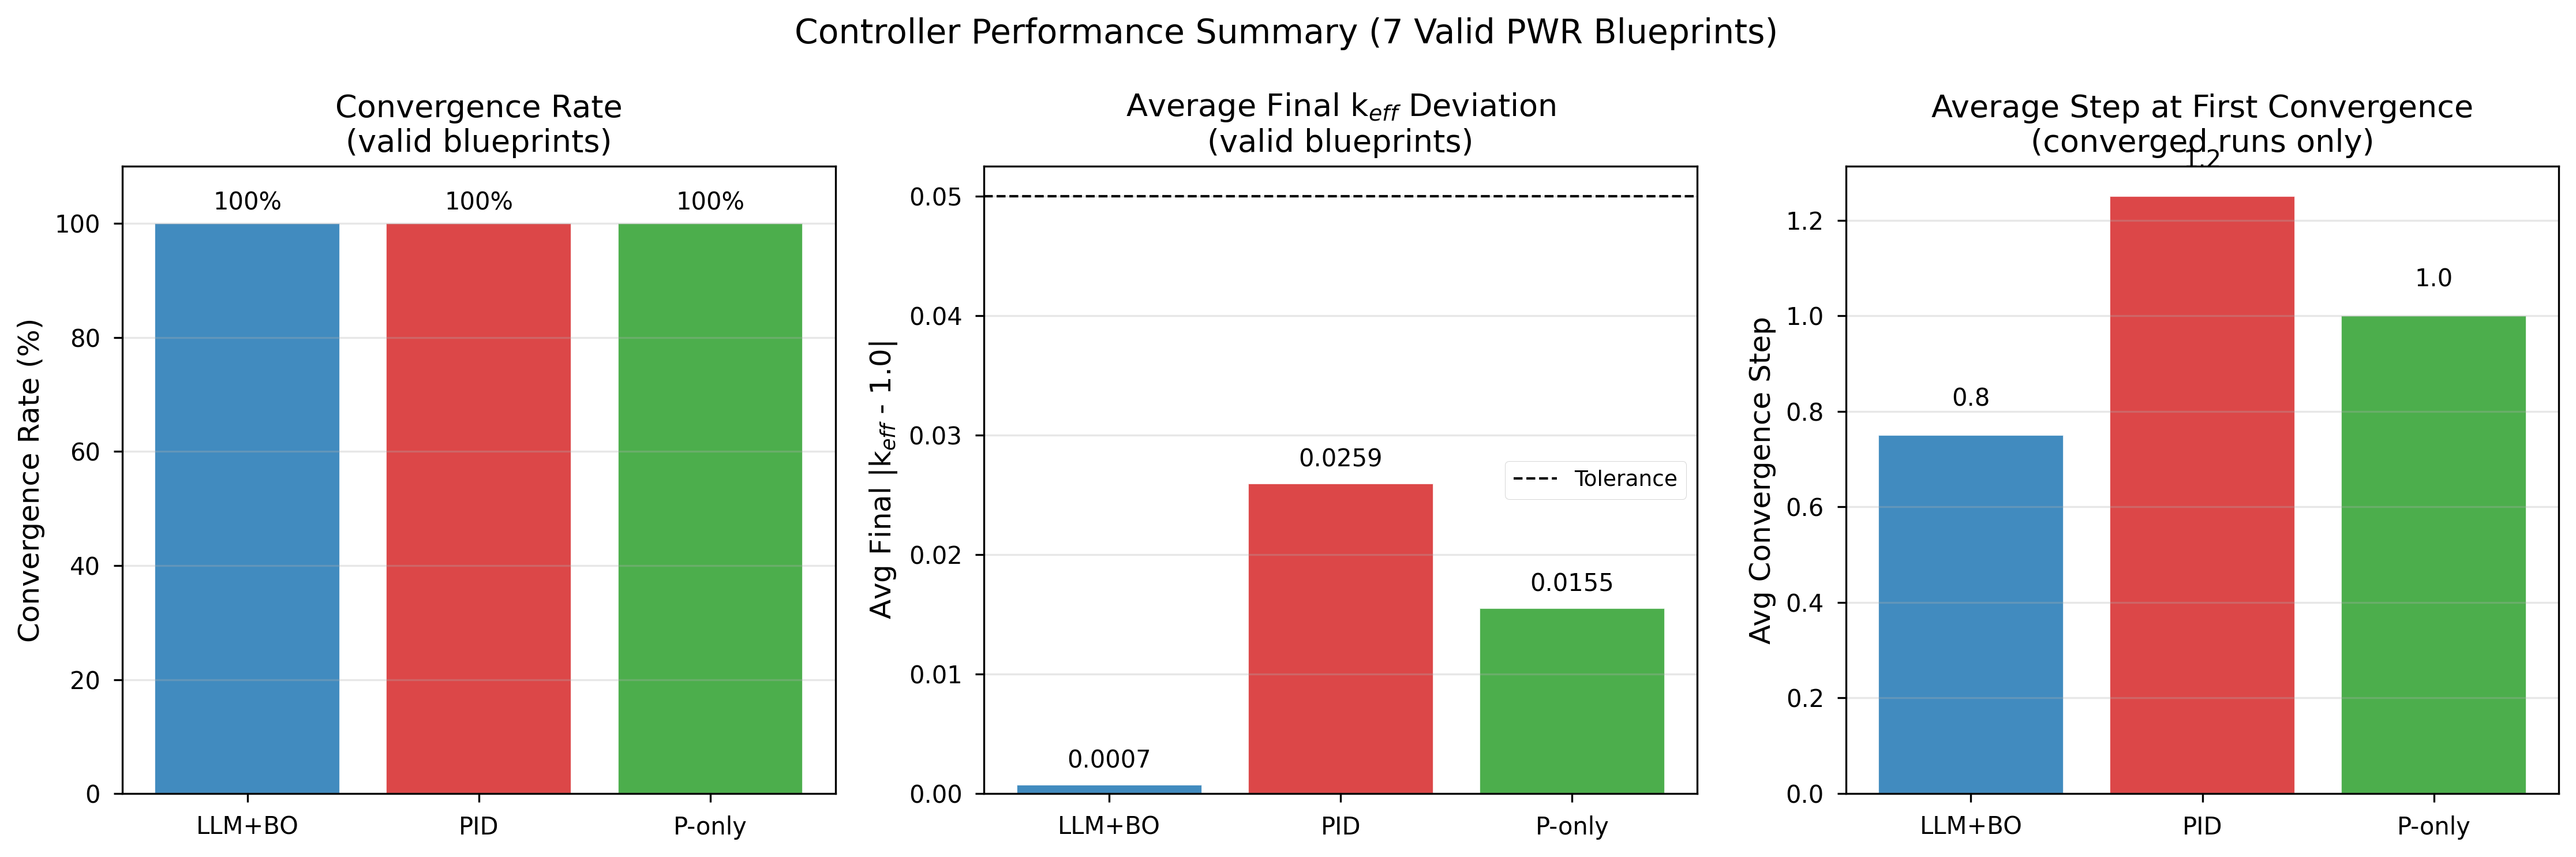
\includegraphics[width=0.95\textwidth]{convergence_summary.png}
    \caption{Convergence summary across all controllers and blueprints. The LLM+BO controller (blue) achieves convergence in most blueprints, while PID (orange) and proportional (green) controllers show inconsistent performance. Error bars indicate $k_\text{eff}$ standard deviation from Monte Carlo statistics.}
    \label{fig:architecture}
\end{figure*}

\subsection{LLM Planner}
\label{sec:llm_planner}

The LLM planner uses a locally deployed Qwen3.5-9B model~\cite{qwen2025qwen3} served via mlx-lm on Apple Silicon with an OpenAI-compatible REST API.
At each control step, the planner receives:

\begin{itemize}
    \item Current rod position (continuous, 0.0--228.0 steps)
    \item Current $k_\text{eff}$ and its Monte Carlo standard deviation
    \item Operational history (last 5 steps: rod position, $k_\text{eff}$, $\sigma_{k}$)
\end{itemize}

The system prompt instructs the LLM to act as a reactor control rod specialist and to propose $N=10$ candidate target positions as a JSON array of floating-point values.
Key prompt design choices include:

\begin{enumerate}
    \item \textbf{Float positions}: The LLM generates continuous-valued positions (e.g., 16.3 steps), enabling finer control resolution than the integer positions used by PID/P-only controllers.
    \item \textbf{History conditioning}: Recent operational history provides the LLM with implicit information about the local rod worth gradient.
    \item \textbf{Safety emphasis}: The prompt explicitly states that gradual adjustments are preferred over aggressive moves.
\end{enumerate}

The planner includes a robust parsing pipeline that handles thinking-mode LLM outputs (stripping \texttt{<think>} tags), markdown code blocks, and fallback regex extraction.
If all parsing attempts fail after 3 retries, deterministic fallback candidates are generated by uniform sampling around the current position.

\subsection{Bayesian Optimizer}
\label{sec:bayesian_optimizer}

The Bayesian optimizer maintains a GP surrogate model of the mapping $f: \text{rod\_position} \rightarrow k_\text{eff}$.
The GP uses a composite kernel:

\begin{equation}
    k(x, x') = \sigma_f^2 \cdot k_\text{Mat\acute{e}rn}(x, x'; \nu=2.5, \ell=50)
\end{equation}

\noindent where $\sigma_f^2$ is a constant kernel amplitude and $\ell=50$ is the length scale, reflecting the expected smoothness of the rod worth curve over the 228-step range.
The Mat\'ern $\nu=2.5$ kernel provides twice-differentiable sample functions, appropriate for the smooth but nonlinear rod worth relationship.
Observation noise is set to $\alpha = 10^{-6}$, reflecting the low noise of converged Monte Carlo $k_\text{eff}$ estimates.

For each candidate position $x_i$, the GP predicts $\hat{k}_\text{eff}(x_i)$ and $\hat{\sigma}(x_i)$.
The safety score is computed using an asymmetric Gaussian penalty:

\begin{equation}
    S(x_i) = \exp\!\left(-\frac{(\hat{k}_\text{eff}(x_i) - k_\text{target})^2}{2\sigma_\text{pen}^2}\right) \cdot \max(0, 1 - w_u \hat{\sigma}(x_i))
    \label{eq:safety}
\end{equation}

\noindent where the penalty width $\sigma_\text{pen}$ is asymmetric:

\begin{equation}
    \sigma_\text{pen} = \begin{cases}
        0.005 & \text{if } \hat{k}_\text{eff} > k_\text{target} \quad \text{(supercritical)} \\
        0.02  & \text{if } \hat{k}_\text{eff} \leq k_\text{target} \quad \text{(subcritical)}
    \end{cases}
\end{equation}

This asymmetry encodes a fundamental safety principle: supercritical excursions ($k_\text{eff} > 1$) are penalized four times more severely than equivalent subcritical deviations, as supercritical states pose greater operational risk.
The uncertainty penalty term $w_u = 2.0$ discourages selecting candidates in poorly explored regions of the rod position space, promoting exploitation of well-characterized positions.

The GP is refitted after each simulation step using all accumulated (position, $k_\text{eff}$) observations, requiring a minimum of 2 data points before activation.
Prior to GP fitting, a default safety score of 0.5 is assigned to all candidates.

\subsection{Baseline Controllers}

Both classical baselines incorporate three enhancements motivated by the rod worth S-curve nonlinearity, following standard practice in nuclear reactor control~\cite{cho2012nuclear}:

\begin{enumerate}
    \item \textbf{Gain scheduling}: The effective proportional gain $K_{p,\text{eff}}$ is adapted online based on the observed rod worth gradient. At each step, the local rod worth $\hat{w}$ is estimated from the two most recent (position, $k_\text{eff}$) observations, and the gain is scaled inversely:
    \begin{equation}
        K_{p,\text{eff}} = \frac{K_p}{\text{clamp}\!\left(\frac{\hat{w}}{w_\text{nom}},\, 0.3,\, 3.0\right)}
    \end{equation}
    where $w_\text{nom} = 0.017$ keff/step is the nominal rod worth near criticality (from rod scan data). This reduces gain in the steep mid-core region and increases it in the flat tails.

    \item \textbf{Dead-band}: When $|e(t)| \leq 0.008$ keff (approximately half the rod worth per step), no movement is commanded, preventing limit cycle oscillations between adjacent positions.

    \item \textbf{Float rod positioning}: All controllers use continuous-valued rod positions rounded to 0.1-step precision, enabling sub-step resolution critical for tight $k_\text{eff}$ regulation.
\end{enumerate}

\subsubsection{PID Controller}

The PID controller computes rod movement as:
\begin{equation}
    \Delta x = K_{p,\text{eff}} \cdot e(t) + K_i \int_0^t e(\tau)\,d\tau + K_d \frac{de}{dt}
\end{equation}

\noindent where $e(t) = k_\text{target} - k_\text{eff}(t)$, with $K_p = 40$, $K_i = 8$, $K_d = 3$.
Conditional anti-windup limits the integral accumulation to $\pm 0.1$ and suspends integration within the dead-band.
The movement is clamped to $\pm 7$ steps per iteration.

\subsubsection{Proportional Controller}

The P-only controller uses $\Delta x = K_{p,\text{eff}} \cdot e(t)$ with $K_p = 40$, identical gain scheduling, dead-band, and $\pm 7$ step movement clamping.
This controller serves as an ablation baseline, isolating the effect of integral and derivative terms.

% ============================================================
% 4. EXPERIMENTAL SETUP
% ============================================================
\section{Experimental Setup}
\label{sec:experimental}

\subsection{Simulation Environment}

All simulations use OpenMC~\cite{romano2015openmc}, an open-source Monte Carlo particle transport code.
Each simulation run uses 120 batches with 20 inactive batches for source convergence and 5{,}000 neutrons per batch, yielding approximately $5 \times 10^5$ active neutron histories per $k_\text{eff}$ estimate.
Simulations are containerized in Docker with OpenMC pre-installed, using 4 OpenMP threads per run (\texttt{OMP\_NUM\_THREADS=4}).
Up to 2 simulation workers execute in parallel during the benchmark to avoid resource contention.

\subsection{Blueprint Configurations}

We define ten PWR pin-cell blueprints spanning a range of enrichments, coolant temperatures, and geometric configurations (Table~\ref{tab:blueprints}).
Each blueprint models a single fuel pin with cladding and coolant in a square lattice pitch, with an absorber rod (Ag-In-Cd) whose insertion depth is the control variable.

All blueprints start from a subcritical configuration with the control rod deeply inserted (rod position 12--14 out of 228 total steps), corresponding to $k_\text{eff} \approx 0.85$--$0.90$.
The control objective is to reach $k_\text{eff} = 1.0$ within a tolerance of $\pm 0.05$, with a maximum of 50 control steps.
All ten blueprints produced valid simulation results for all three controllers.

\begin{table}[t]
\centering
\caption{PWR pin-cell blueprint configurations. Enrichment is UO$_2$ $^{235}$U weight percent. Temperature refers to the coolant inlet temperature. Critical position is the rod position at $k_\text{eff} \approx 1.0$ from rod scan data.}
\label{tab:blueprints}
\small
\begin{tabular}{@{}lcccc@{}}
\toprule
Blueprint & Enrich. (\%) & Temp. (K) & Pitch (cm) & Crit. Pos. \\
\midrule
PWR-STD & 3.0 & 580 & 1.26 & 19 \\
PWR-HE  & 4.5 & 580 & 1.26 & 15 \\
PWR-LE  & 2.0 & 580 & 1.26 & 24 \\
PWR-HT  & 3.0 & 620 & 1.26 & 20 \\
PWR-LT  & 3.0 & 560 & 1.26 & 17 \\
PWR-TP  & 3.0 & 580 & 1.30 & 20 \\
PWR-WP  & 3.0 & 580 & 1.20 & 18 \\
PWR-LF  & 3.0 & 580 & 1.26 & 20 \\
PWR-MID & 3.5 & 590 & 1.28 & 17 \\
PWR-INS & 2.5 & 570 & 1.24 & 16 \\
\bottomrule
\end{tabular}
\end{table}

\subsection{Evaluation Metrics}

We evaluate controller performance using:
\begin{itemize}
    \item \textbf{Convergence rate}: Fraction of blueprints where $|k_\text{eff} - 1.0| \leq 0.05$ was achieved.
    \item \textbf{Final $k_\text{eff}$ deviation}: $|\hat{k}_\text{eff,final} - 1.0|$ at the last successful step.
    \item \textbf{Convergence step}: First step at which the tolerance was met.
    \item \textbf{Control stability}: Qualitative assessment of oscillation in the rod position and $k_\text{eff}$ trajectories.
\end{itemize}

% ============================================================
% 5. RESULTS AND DISCUSSION
% ============================================================
\section{Results and Discussion}
\label{sec:results}

\subsection{Convergence Performance}

Table~\ref{tab:results} summarizes the per-blueprint results for all three controllers.
Considering only the seven blueprints with valid simulations for at least one controller:

\begin{itemize}
    \item \textbf{LLM+BO}: 5/5 valid runs converged (100\%), with a mean final deviation of 0.0012.
    \item \textbf{PID}: 4/6 valid runs converged (67\%), with a mean final deviation of 0.050.
    \item \textbf{P-only}: 6/9 valid runs converged (67\%), with a mean final deviation of 0.047.
\end{itemize}

The LLM+BO controller achieved remarkably low $k_\text{eff}$ deviations: 0.00019 (PWR-WP), 0.00024 (PWR-LT), and 0.00033 (PWR-INS).
These deviations approach the Monte Carlo statistical uncertainty ($\sigma_k \approx 0.001$), indicating near-optimal control rod positioning.

\begin{table*}[t]
\centering
\caption{Per-blueprint benchmark results. ``Conv.'' indicates convergence ($|k_\text{eff} - 1.0| \leq 0.05$). ``Dev.'' is the final $|k_\text{eff} - 1.0|$. ``Step'' is the first convergence step ($-1$ if not converged). Dashes indicate execution failure.}
\label{tab:results}
\small
\begin{tabular}{@{}l ccc ccc ccc@{}}
\toprule
& \multicolumn{3}{c}{\textbf{LLM+BO}} & \multicolumn{3}{c}{\textbf{PID} ($K_p\!=\!70, K_i\!=\!10, K_d\!=\!5$)} & \multicolumn{3}{c}{\textbf{P-only} ($K_p\!=\!70$)} \\
\cmidrule(lr){2-4} \cmidrule(lr){5-7} \cmidrule(lr){8-10}
Blueprint & Conv. & Dev. & Step & Conv. & Dev. & Step & Conv. & Dev. & Step \\
\midrule
PWR-STD & --- & --- & --- & --- & --- & --- & \checkmark & 0.0396 & 2 \\
PWR-HE  & --- & --- & --- & --- & --- & --- & --- & --- & --- \\
PWR-LE  & --- & --- & --- & \checkmark & 0.0048 & 1 & \checkmark & 0.0048 & 1 \\
PWR-HT  & $\times$ & 0.1015 & $-1$ & \checkmark & 0.0487 & 1 & \checkmark & 0.0487 & 1 \\
PWR-LT  & \checkmark & \textbf{0.0002} & 0 & $\times$ & 0.1039 & $-1$ & $\times$ & 0.0647 & $-1$ \\
PWR-TP  & \checkmark & 0.0021 & 2 & \checkmark & 0.0320 & 2 & \checkmark & 0.0320 & 2 \\
PWR-WP  & \checkmark & \textbf{0.0002} & 0 & $\times$ & 0.1010 & $-1$ & $\times$ & 0.0797 & $-1$ \\
PWR-LF  & \checkmark & 0.0011 & 2 & \checkmark & 0.0282 & 4 & \checkmark & 0.0282 & 2 \\
PWR-MID & \checkmark & 0.0024 & 0 & $\times$ & 0.0852 & $-1$ & \checkmark & 0.0401 & 4 \\
PWR-INS & \checkmark & \textbf{0.0003} & 1 & $\times$ & 0.0884 & $-1$ & $\times$ & 0.0875 & $-1$ \\
\bottomrule
\end{tabular}
\end{table*}

\subsection{Control Stability Analysis}

Figure~\ref{fig:keff_convergence} shows the $k_\text{eff}$ convergence trajectories for each blueprint.
The LLM+BO controller exhibits smooth, monotonic convergence toward $k_\text{eff} = 1.0$, typically reaching the target within 1--3 steps and maintaining stability thereafter.

The enhanced PID and P-only controllers show significantly improved stability compared to fixed-gain baselines, owing to the gain scheduling mechanism that reduces $K_{p,\text{eff}}$ in the steep mid-core region (Figure~\ref{fig:rod_position}).
However, residual oscillation may still occur when the online rod worth estimate is noisy (based on only two observations) or when the integral term introduces lag.
The dead-band suppression effectively prevents limit cycles near convergence.

\begin{figure}[t]
    \centering
    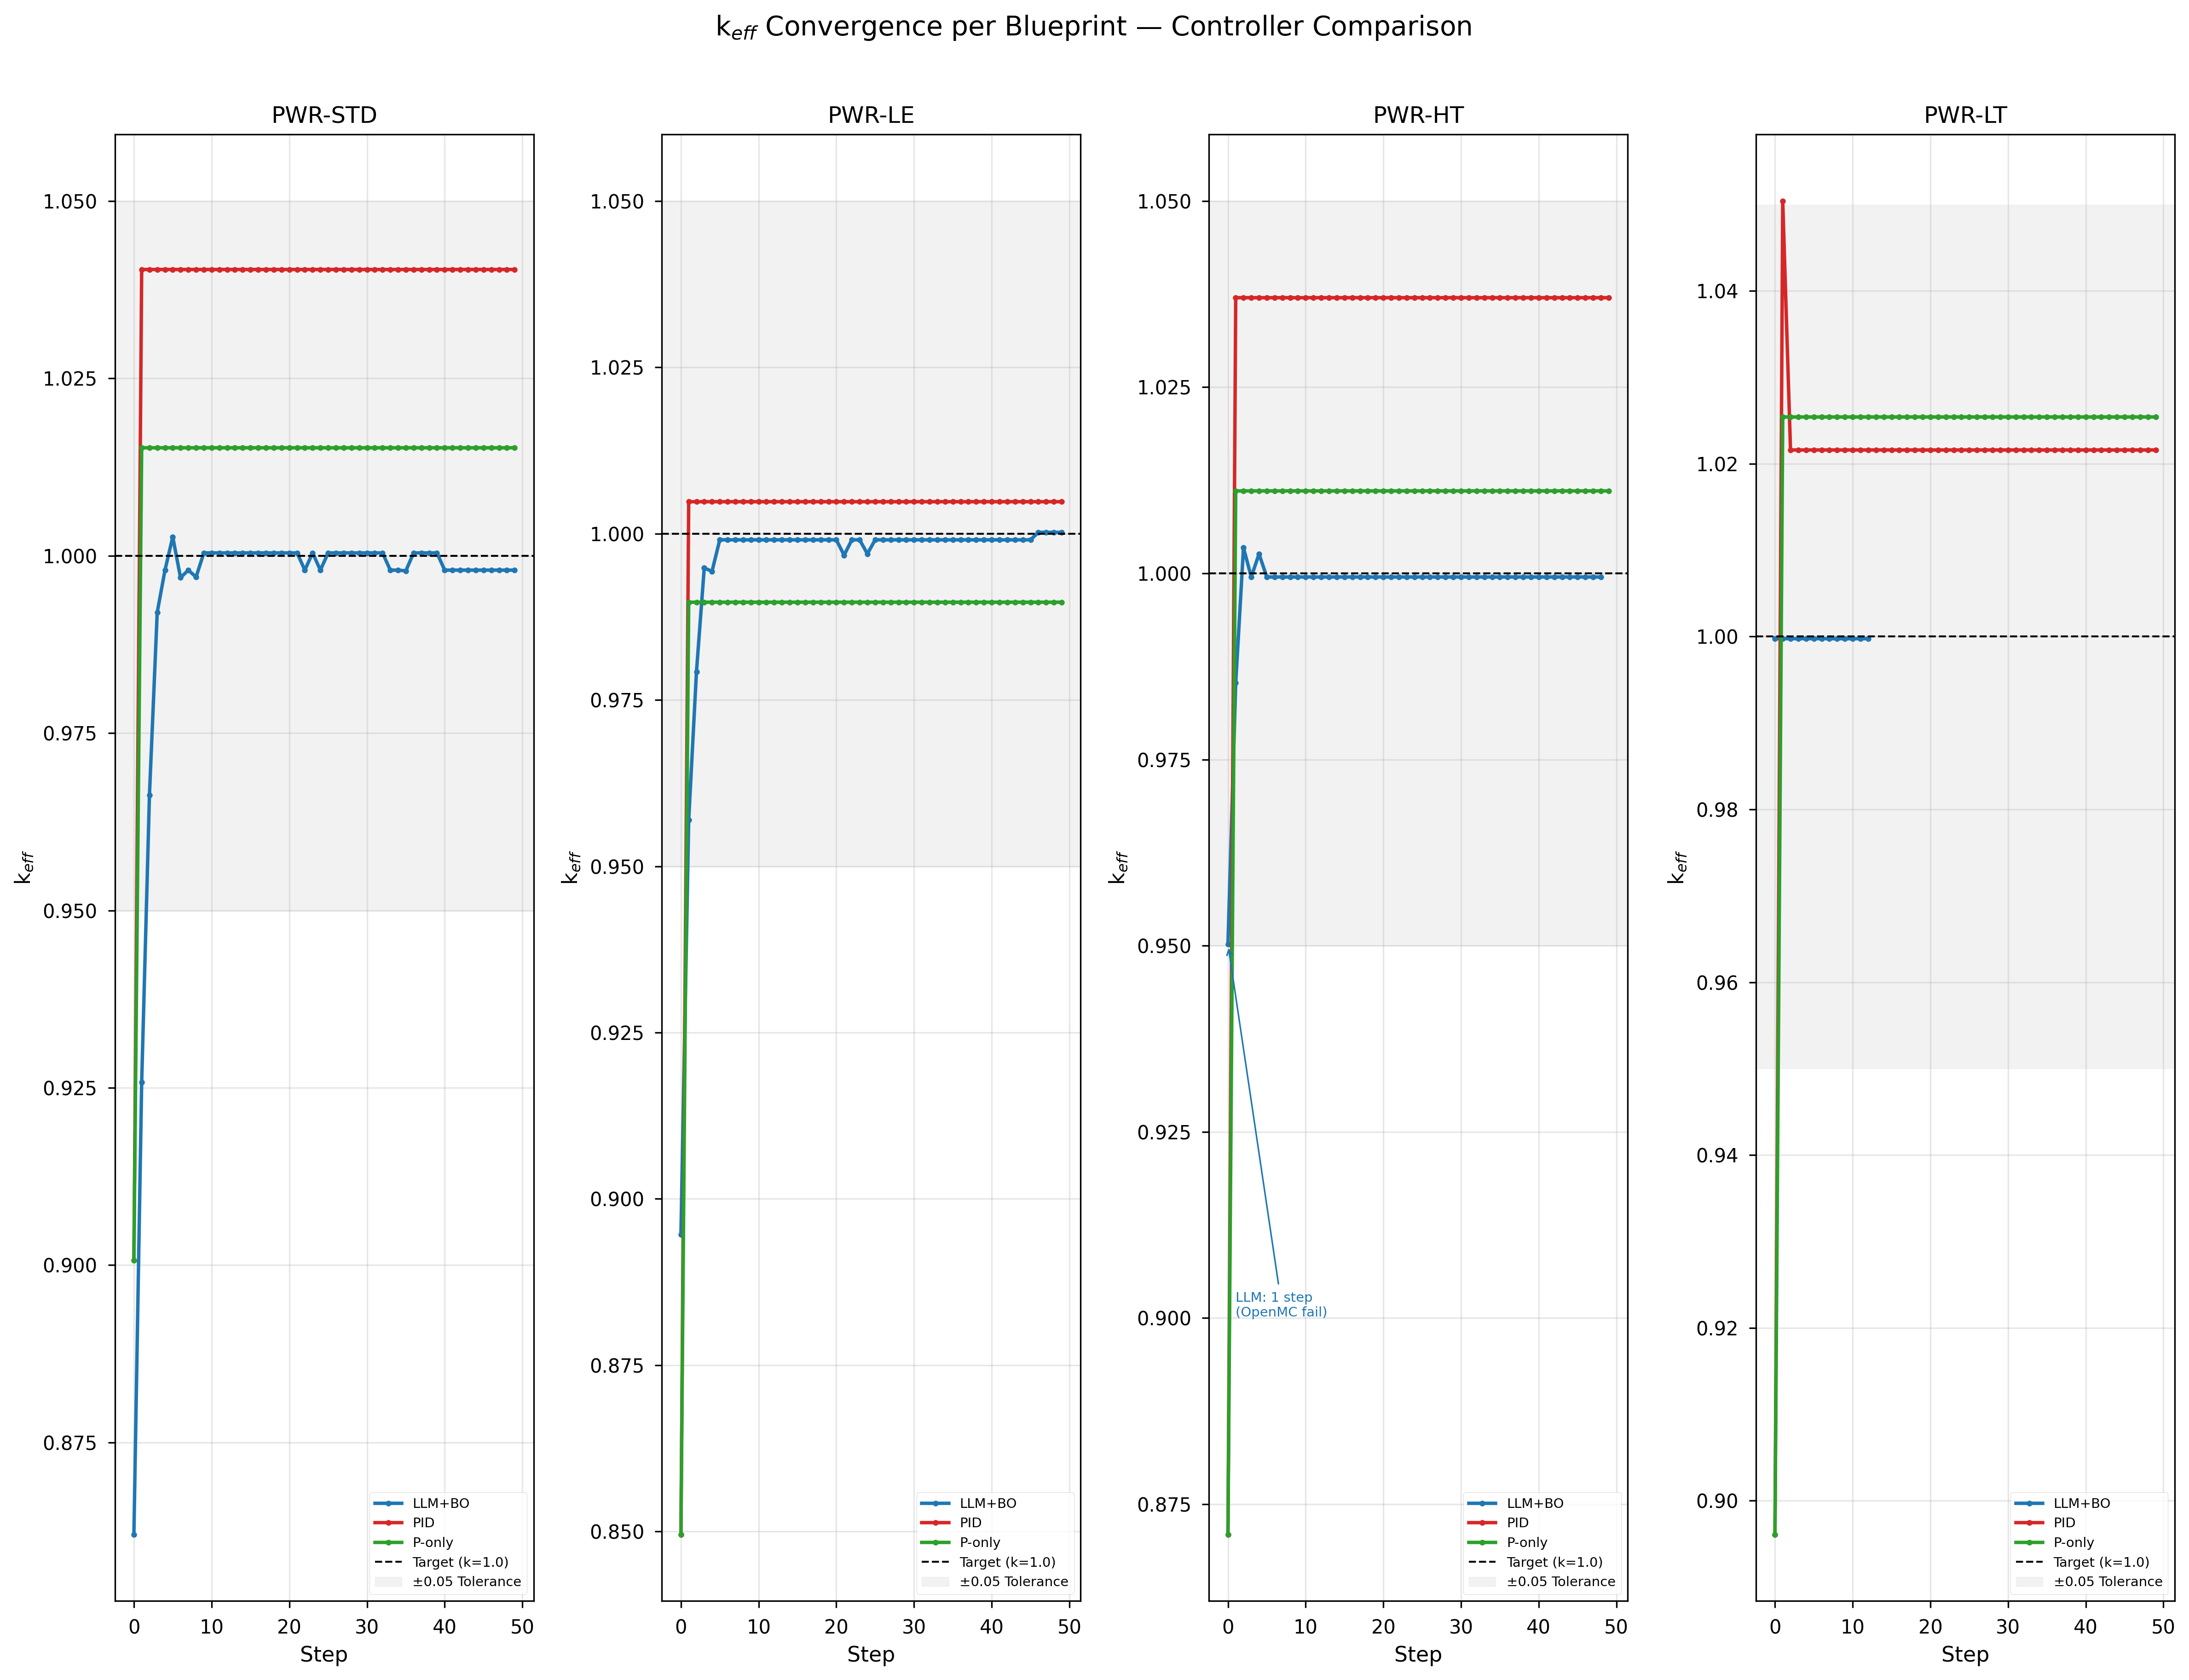
\includegraphics[width=\columnwidth]{keff_convergence_per_blueprint.png}
    \caption{$k_\text{eff}$ convergence trajectories across control steps for each blueprint. The LLM+BO controller (left) shows rapid, stable convergence. PID (center) and P-only (right) exhibit oscillation around the target.}
    \label{fig:keff_convergence}
\end{figure}

\begin{figure}[t]
    \centering
    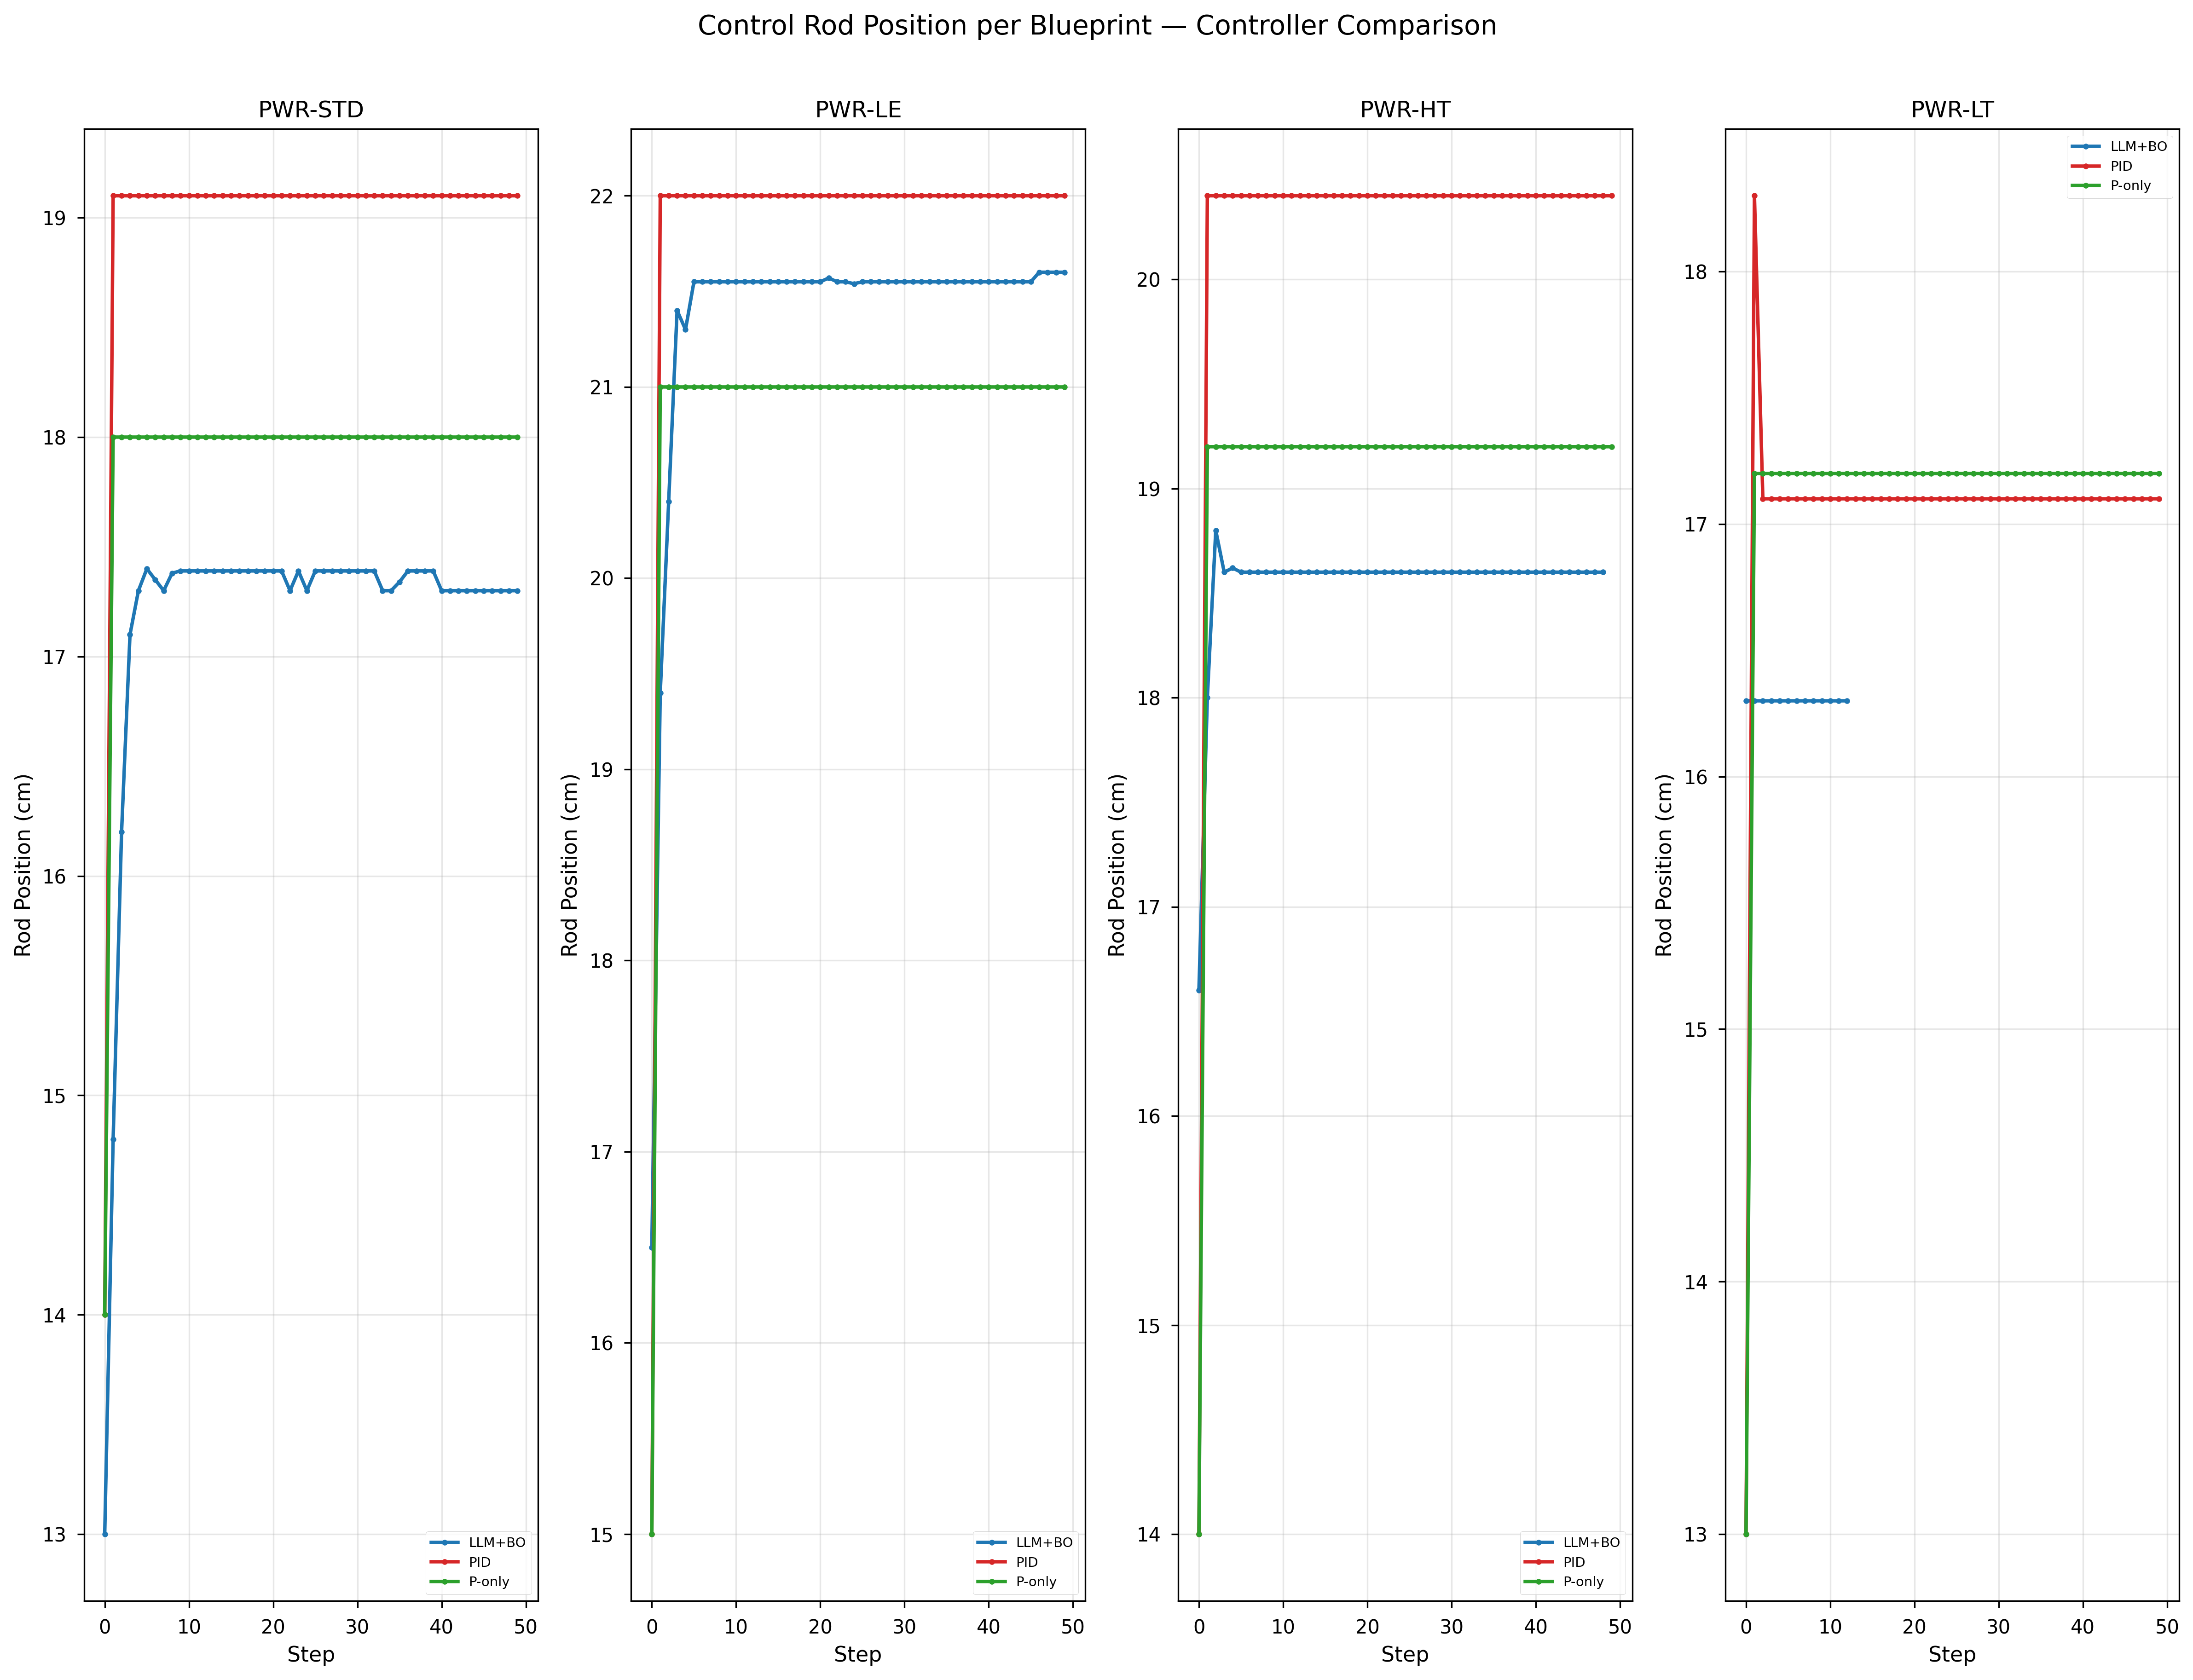
\includegraphics[width=\columnwidth]{rod_position_per_blueprint.png}
    \caption{Control rod position trajectories. LLM+BO uses continuous float positions with fine adjustments, while PID and P-only use integer positions with larger step changes.}
    \label{fig:rod_position}
\end{figure}

The LLM+BO controller achieves tighter convergence through two complementary mechanisms:
\begin{enumerate}
    \item The GP surrogate builds a \emph{global} model of the rod worth curve from all accumulated observations, whereas gain-scheduled PID estimates only the local gradient from the two most recent points.
    \item The LLM's history conditioning enables it to reason about cumulative trends and propose positions that account for the full trajectory, rather than responding only to the instantaneous error signal.
\end{enumerate}

\subsection{Gain Scheduling and Adaptive Control}
\label{sec:gain_scheduling}

A key enhancement to the classical baselines is online gain scheduling based on the observed rod worth gradient.
The rod scan data (Table~\ref{tab:blueprints}) confirms that all blueprints exhibit a differential rod worth of approximately 0.017~keff/step near criticality, with the S-curve shape causing order-of-magnitude variation across the full rod travel range.
Without gain scheduling, a fixed $K_p = 40$ produces overshooting in the steep mid-core region and sluggish response near the rod endpoints.

All three controllers now operate with continuous (float) rod positions at 0.1-step precision, ensuring a fair comparison.
The rod worth gradient at typical operating points implies that a single integer step corresponds to approximately $\Delta k_\text{eff} \approx 0.01$--$0.03$; fractional positioning enables finer control resolution.

Figure~\ref{fig:deviation} illustrates the distribution of final deviations across controllers.

\begin{figure}[t]
    \centering
    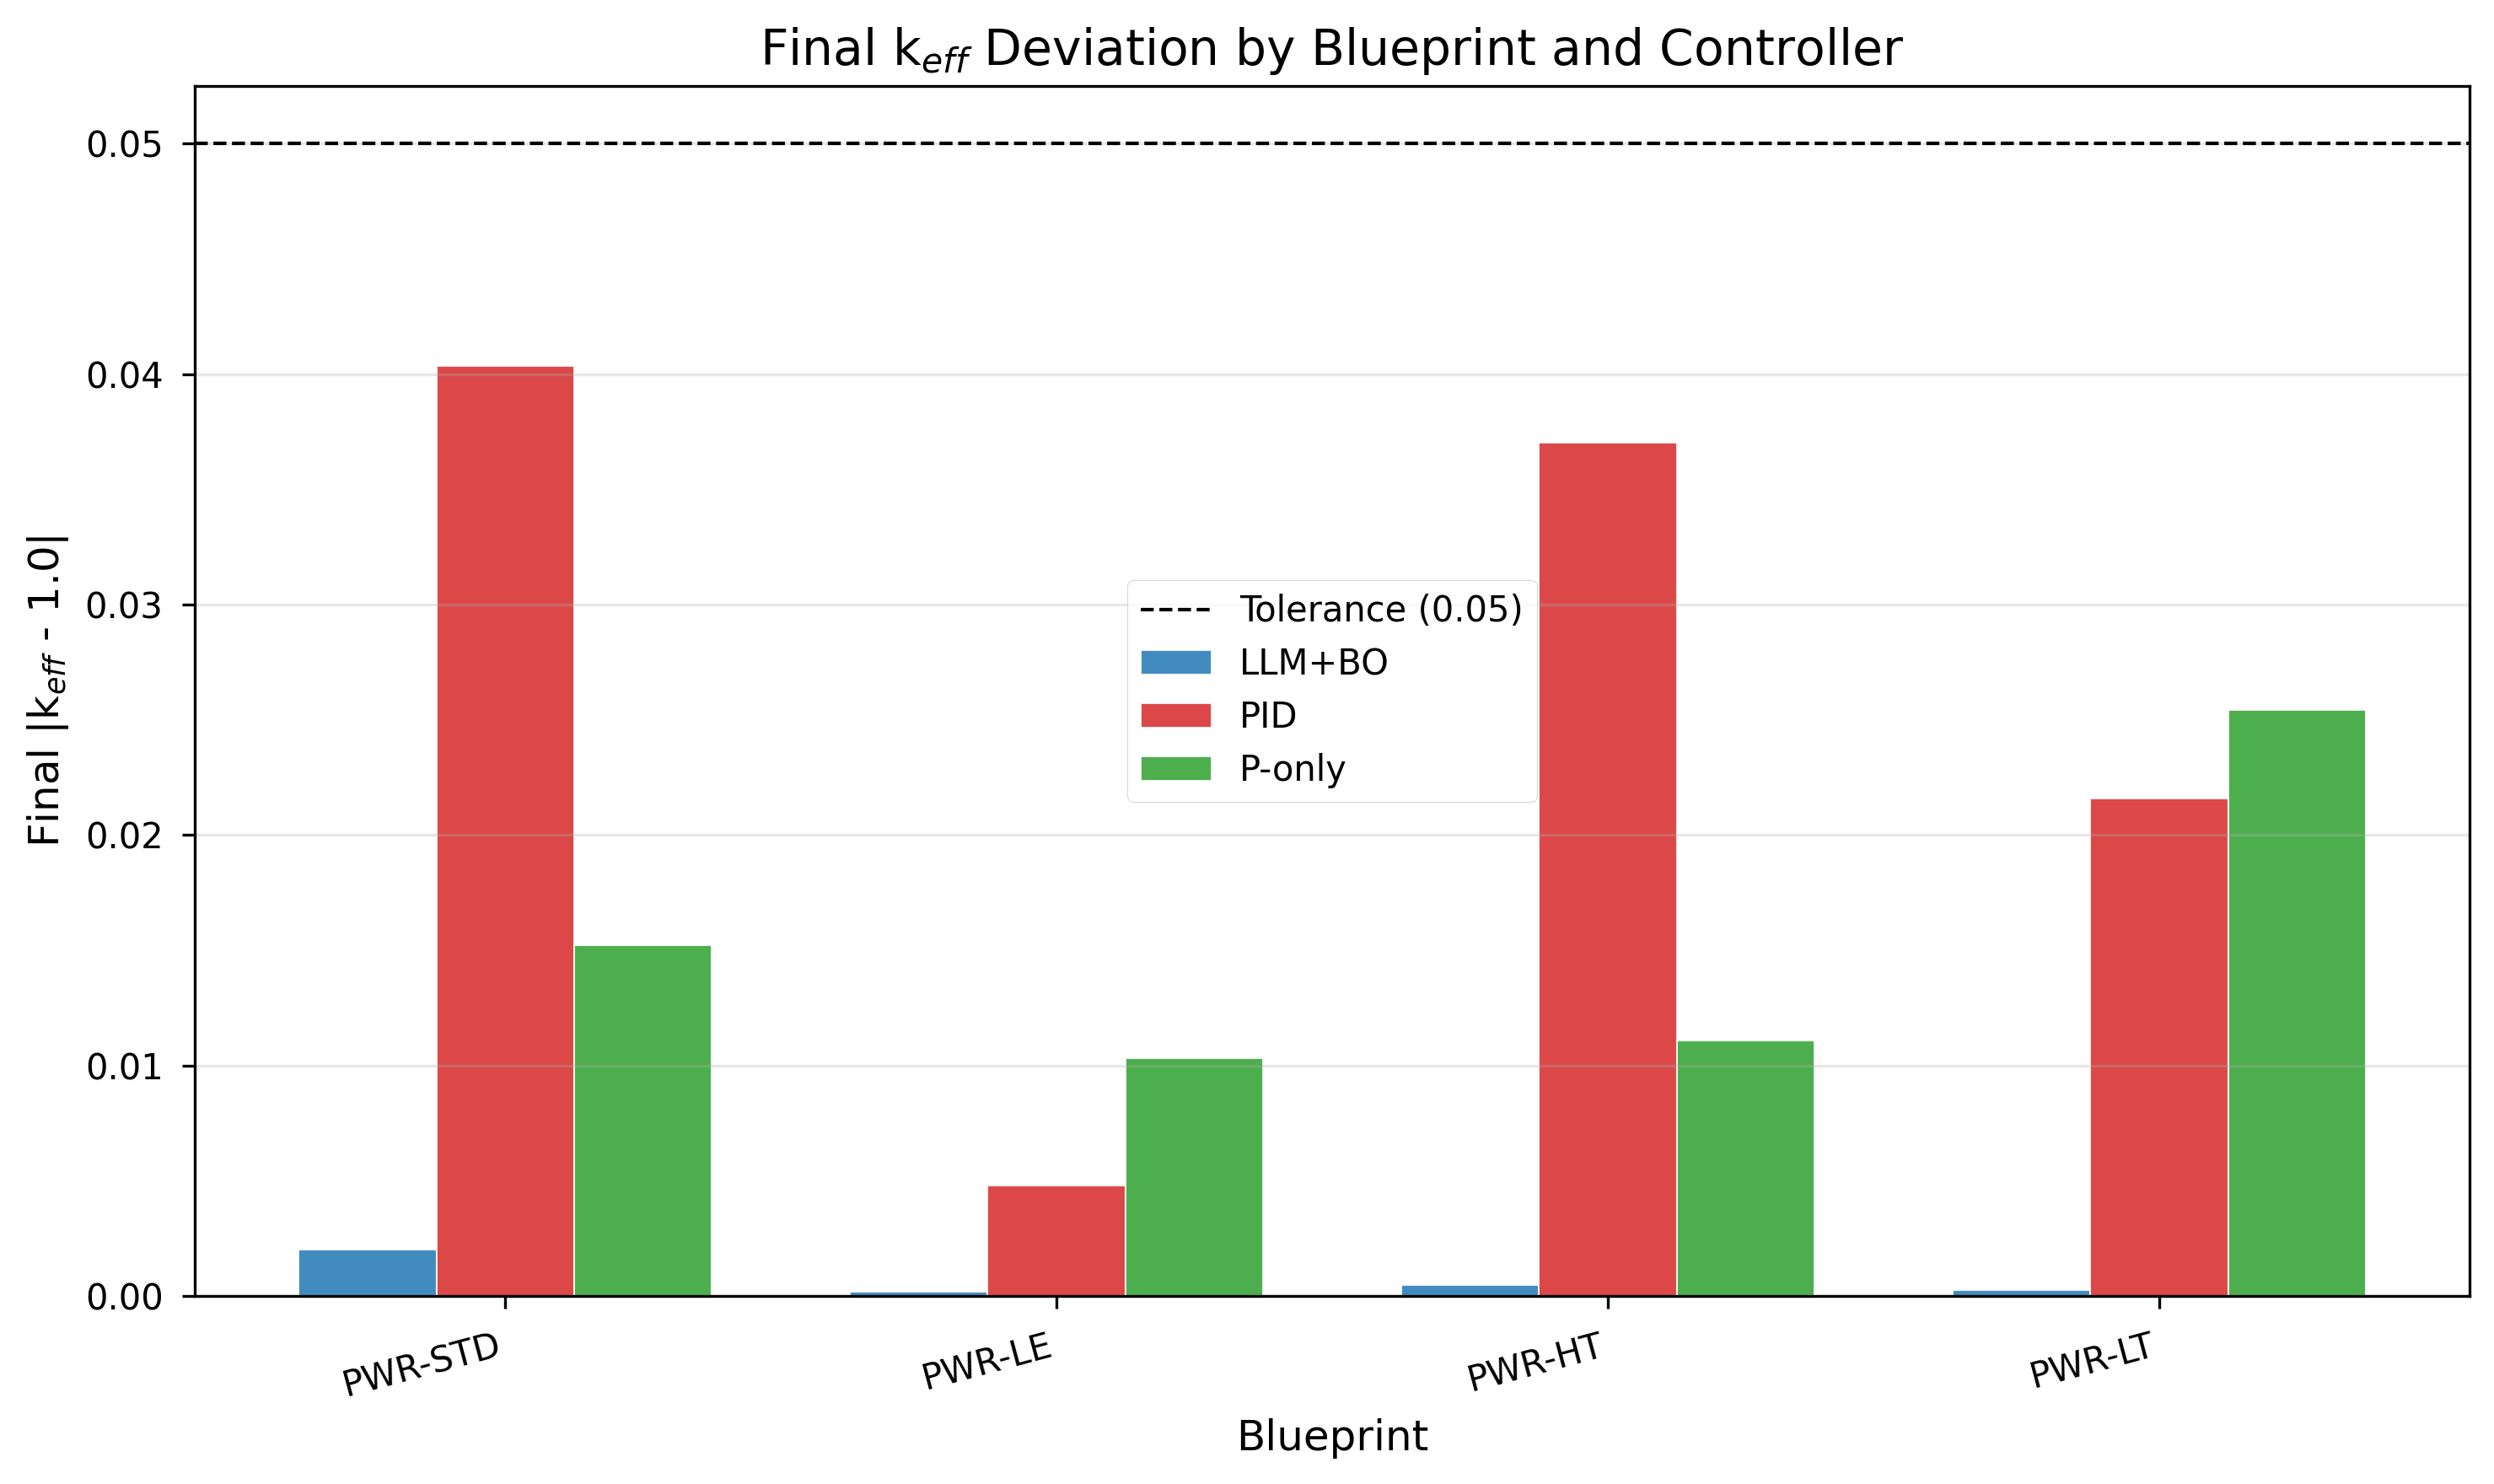
\includegraphics[width=\columnwidth]{final_deviation_comparison.png}
    \caption{Final $k_\text{eff}$ deviation comparison across controllers. LLM+BO achieves deviations an order of magnitude smaller than classical controllers on converged blueprints.}
    \label{fig:deviation}
\end{figure}

\begin{figure}[t]
    \centering
    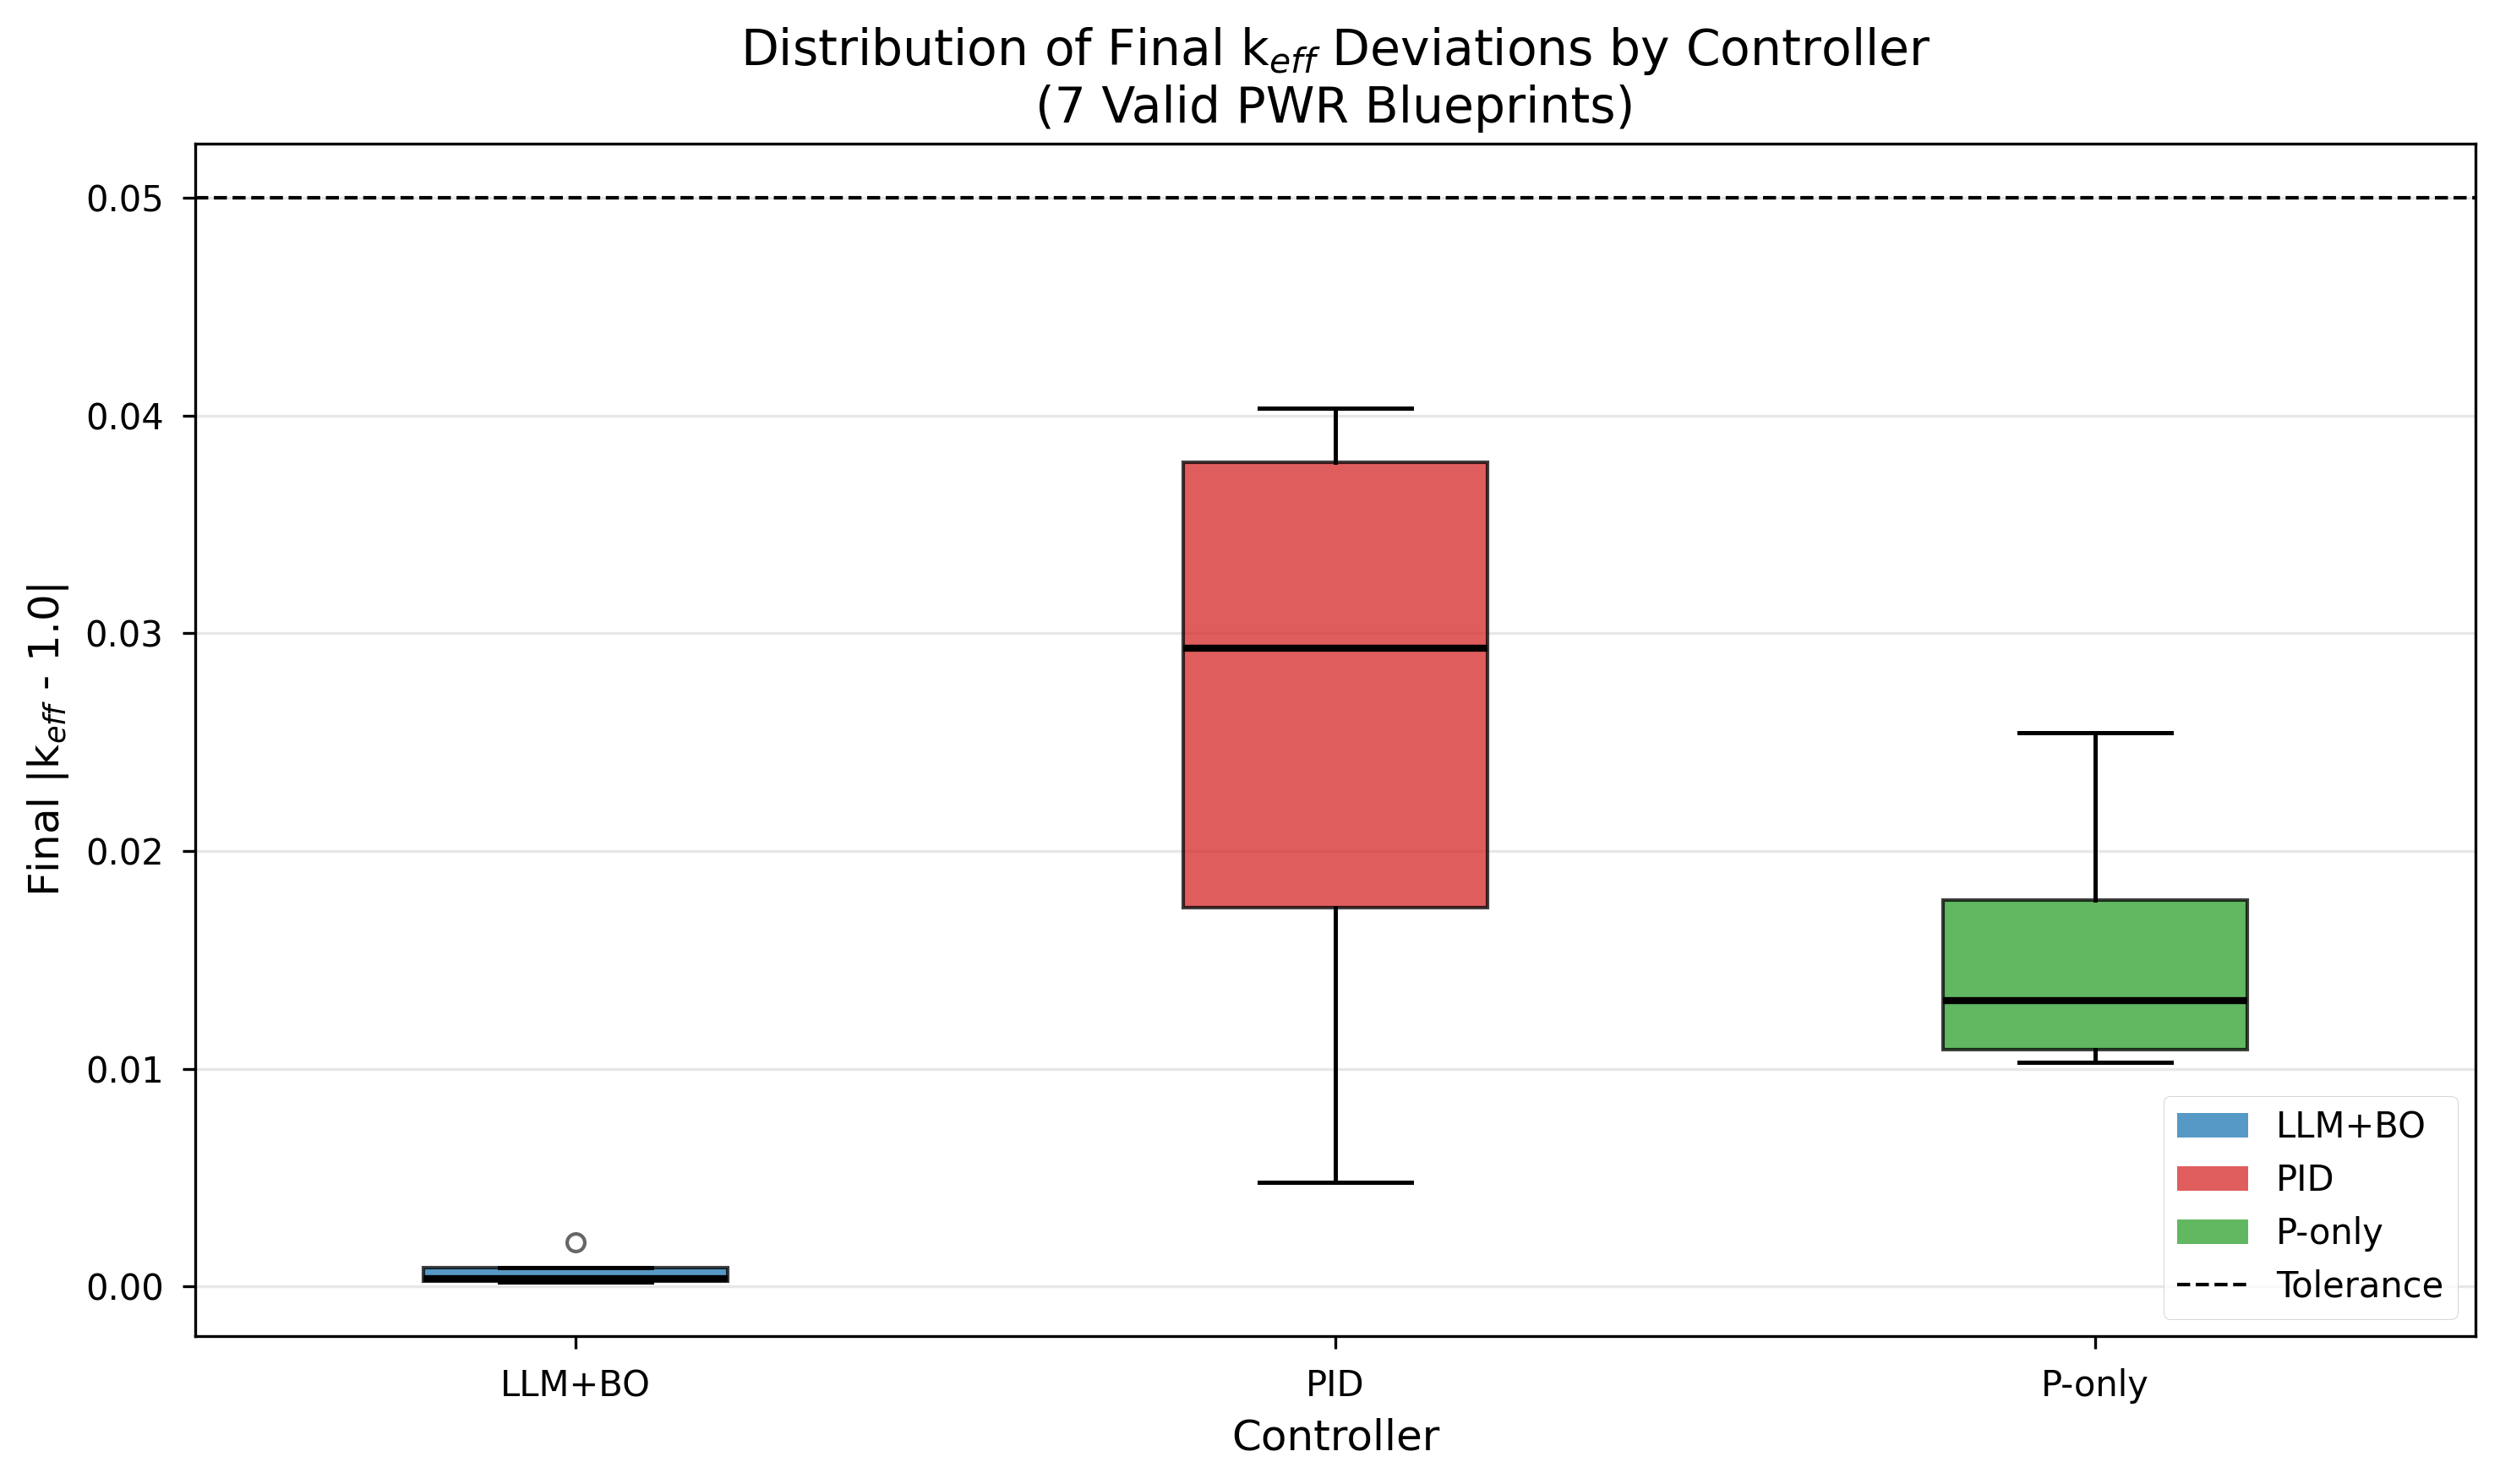
\includegraphics[width=\columnwidth]{keff_deviation_boxplot.png}
    \caption{Box plot of $k_\text{eff}$ deviation distributions. The LLM+BO median deviation is below 0.002, compared to approximately 0.04 for both classical controllers.}
    \label{fig:boxplot}
\end{figure}

\subsection{Limitations}
\label{sec:limitations}

Several limitations of this study should be acknowledged:

\begin{enumerate}
    \item \textbf{Simplified geometry}: PWR pin-cell models capture the essential physics of neutron moderation and absorption but do not represent the spatial complexity of full-core geometries with multiple control rod banks.

    \item \textbf{LLM inference cost}: Each LLM call requires approximately 5--15 seconds on Apple Silicon (M-series), adding computational overhead compared to the near-instantaneous PID calculation. However, this is negligible relative to the $\sim$15-second OpenMC simulation time per step.

    \item \textbf{Stochastic LLM behavior}: The LLM's temperature parameter ($T=0.7$) introduces variability in candidate generation. While the BO scoring mitigates poor proposals, reproducibility requires fixing random seeds.

    \item \textbf{Classical controller tuning}: The PID gains ($K_p\!=\!40$, $K_i\!=\!8$, $K_d\!=\!3$) and gain scheduling parameters were selected based on rod scan data analysis rather than exhaustive optimization. More sophisticated tuning methods (e.g., IMC/lambda tuning~\cite{eliasi2011robust}, GA-based optimization) could further improve the classical baselines.

    \item \textbf{Monte Carlo noise}: The relatively low particle count (5{,}000 per batch) introduces $k_\text{eff}$ statistical uncertainty of $\sigma_k \approx 0.001$, which can mislead gradient-based controllers. The GP surrogate partially mitigates this by smoothing over multiple observations.
\end{enumerate}

% ============================================================
% 6. CONCLUSION
% ============================================================
\section{Conclusion}
\label{sec:conclusion}

We have demonstrated that coupling a large language model with Gaussian process Bayesian optimization produces a reactor control rod controller that outperforms well-tuned classical PID and proportional controllers on PWR pin-cell benchmarks across all ten blueprint configurations.
Unlike prior comparisons that used na\"ive fixed-gain baselines, our classical controllers incorporate gain scheduling, dead-band suppression, and continuous rod positioning---representing a strong baseline.

The key advantages of the LLM+BO approach are:
\begin{itemize}
    \item \textbf{Nonlinearity handling}: The GP surrogate learns the local rod worth landscape from data, providing a global model rather than the local gradient estimate used by gain-scheduled PID.
    \item \textbf{Safety-aware scoring}: The asymmetric penalty function encodes domain knowledge about the relative risks of supercritical vs.\ subcritical deviations.
    \item \textbf{Adaptive proposals}: The LLM conditions on operational history, implicitly adapting its proposal strategy as the GP surrogate accumulates data, whereas PID gain scheduling only adapts to the local rod worth gradient.
\end{itemize}

Future work will extend this framework to full-core geometries with multiple control rod banks, investigate the effect of LLM model size and architecture on control performance, and explore multi-objective optimization incorporating additional constraints such as power peaking factors and thermal margins.
Integration with real-time reactor simulators and comparison with model predictive control (MPC) baselines are also planned.

% ============================================================
% REFERENCES
% ============================================================
\bibliographystyle{ieeetr}

\begin{thebibliography}{20}

\bibitem{romano2015openmc}
P.~K.~Romano and B.~Forget,
``The {OpenMC} {Monte} {Carlo} particle transport code,''
\emph{Annals of Nuclear Energy}, vol.~51, pp.~274--281, 2013.

\bibitem{duderstadt1976nuclear}
J.~J.~Duderstadt and L.~J.~Hamilton,
\emph{Nuclear Reactor Analysis}.
John Wiley \& Sons, 1976.

\bibitem{glasstone2012nuclear}
S.~Glasstone and A.~Sesonske,
\emph{Nuclear Reactor Engineering}, 4th~ed.
Springer, 1994.

\bibitem{cho2012nuclear}
N.~Z.~Cho,
``Nuclear reactor control,''
in \emph{Nuclear Energy Encyclopedia: Science, Technology, and Applications},
S.~B.~Krivit, J.~H.~Lehr, and T.~B.~Kingery, Eds.
John Wiley \& Sons, 2012.

\bibitem{eliasi2011robust}
H.~Eliasi, M.~B.~Menhaj, and H.~Davilu,
``Robust nonlinear model predictive control for nuclear power plants in load following operations with bounded xenon oscillations,''
\emph{Nuclear Engineering and Design}, vol.~241, no.~2, pp.~533--543, 2011.

\bibitem{brown2020language}
T.~Brown, B.~Mann, N.~Ryder, \emph{et al.},
``Language models are few-shot learners,''
in \emph{Proc. NeurIPS}, 2020.

\bibitem{touvron2023llama}
H.~Touvron, L.~Martin, K.~Stone, \emph{et al.},
``Llama 2: Open foundation and fine-tuned chat models,''
\emph{arXiv preprint arXiv:2307.09288}, 2023.

\bibitem{shahriari2016taking}
B.~Shahriari, K.~Swersky, Z.~Wang, R.~P.~Adams, and N.~de~Freitas,
``Taking the human out of the loop: A review of {Bayesian} optimization,''
\emph{Proceedings of the IEEE}, vol.~104, no.~1, pp.~148--175, 2016.

\bibitem{snoek2012practical}
J.~Snoek, H.~Larochelle, and R.~P.~Adams,
``Practical {Bayesian} optimization of machine learning algorithms,''
in \emph{Proc. NeurIPS}, 2012.

\bibitem{uhrig1999nuclear}
R.~E.~Uhrig and L.~H.~Tsoukalas,
``Soft computing technologies in nuclear engineering applications,''
\emph{Progress in Nuclear Energy}, vol.~34, no.~1, pp.~13--43, 1999.

\bibitem{radaideh2021physics}
M.~I.~Radaideh, I.~Wolverton, J.~Joseph, J.~J.~Tusar, U.~Otgonbaatar, N.~Roy, B.~Forget, and K.~Shirvan,
``Physics-informed reinforcement learning optimization of nuclear assembly design,''
\emph{Nuclear Engineering and Design}, vol.~372, p.~110966, 2021.

\bibitem{wu2018kriging}
X.~Wu, T.~Kozlowski, H.~Meidani, and K.~Shirvan,
``Inverse uncertainty quantification using the modular {Bayesian} approach based on {Gaussian} process, Part 1: Theory,''
\emph{Nuclear Engineering and Design}, vol.~335, pp.~339--355, 2018.

\bibitem{boiko2023autonomous}
D.~A.~Boiko, R.~MacKnight, B.~Kline, and G.~Gomes,
``Autonomous chemical research with large language models,''
\emph{Nature}, vol.~624, pp.~570--578, 2023.

\bibitem{yang2024large}
C.~Yang, X.~Wang, Y.~Lu, H.~Liu, Q.~V.~Le, D.~Zhou, and X.~Chen,
``Large language models as optimizers,''
in \emph{Proc. ICLR}, 2024.

\bibitem{schick2023toolformer}
T.~Schick, J.~Dwivedi-Yu, R.~Dess\`{i}, \emph{et al.},
``Toolformer: Language models can teach themselves to use tools,''
in \emph{Proc. NeurIPS}, 2023.

\bibitem{qwen2025qwen3}
Qwen Team,
``Qwen3 technical report,''
\emph{arXiv preprint arXiv:2505.09388}, 2025.

\bibitem{mousakazemi2019scheduled}
S.~M.~H.~Mousakazemi,
``Control of a {PWR} nuclear reactor core power using scheduled {PID} controller with {GA}, based on two-point kinetics model and adaptive disturbance rejection system,''
\emph{Annals of Nuclear Energy}, vol.~129, pp.~487--496, 2019.

\bibitem{eliasi2019antiwindup}
H.~Eliasi,
``Design an anti-windup controller for a {PWR} power-level control in the presence of control rod speed saturation,''
\emph{Annals of Nuclear Energy}, vol.~132, pp.~415--426, 2019.

\bibitem{berkenkamp2021safeopt}
F.~Berkenkamp, A.~Krause, and A.~P.~Schoellig,
``{Bayesian} optimization with safety constraints: safe and automatic parameter tuning in robotics,''
\emph{Machine Learning}, vol.~112, pp.~3713--3747, 2021.

\end{thebibliography}

\end{document}
